\documentclass[a4paper, ngerman, 12pt, usenames, dvipsnames]{article}
\usepackage[utf8]{inputenc}
\usepackage[ngerman]{babel}
\usepackage[T1]{fontenc}
\usepackage{float}
\usepackage{lmodern}
\usepackage{microtype}
%\usepackage[hidelinks]{hyperref}
\usepackage{hyperref}
\usepackage{url}
\usepackage{graphicx}
\usepackage[dvipsnames]{xcolor}
\usepackage{caption}
\usepackage{subcaption}
\usepackage[export]{adjustbox}
\usepackage{tikzpagenodes}
\usepackage{natbib}
\usetikzlibrary{calc}
\usepackage{fancyhdr}
\usepackage{amssymb}
\usepackage{amsmath}


\title{Aristocracy, Democracy and System Design}
\author{Jasin Aferkou and Egzon Islami}
\date{14. November 2022}

%Page Style
\pagestyle{fancy}
\fancyhf{} % clear all header and footer fields
\renewcommand{\headrulewidth}{0.4pt} % Obere Trennlinie
\fancyfoot[C]{\thepage} 
\fancyhead[R]{Qualitätssicherung}
\fancyhead[L]{\leftmark}
\setlength{\footskip}{50pt}


\begin{document}
\begin{titlepage}

    \begin{figure}[h]
        \begin{subfigure}[t]{10cm}
            \vskip 0pt
            
\includegraphics[width=5cm,left]{images/HKA_IWI_Wortmarke_RGB.jpg}\\
            Studiengang\\
            \textbf{Medien- und Kommunikationsinformatik}\\
            und\\
            \textbf{Informatik}\\
        \end{subfigure}
        \begin{subfigure}[t]{3cm}
            \vskip 0pt
            
\includegraphics[width=3cm,right]{images/HKA_IWI_Bildmarke_RGB.jpg}
        \end{subfigure}
    \end{figure}
    \begin{center}
        %\vspace*{2cm}
        \Large
        \vspace{1cm}
        \huge
        \textbf{Aristocracy, Democracy and System Design}\\
        \vspace{2cm}
        \normalsize
        \textbf{Jasin Aferkou} - 71963 - afja1011@h-ka.de\\
        \textbf{Egzon Islami} - 65124 - iseg1011@h-ka.de\\
        
        \vspace{2cm}
        Qualitätssicherung\\
        \vspace{1.5cm}
        \small
        14. November 2022
    \end{center}
\end{titlepage}
\pagebreak

\tableofcontents
\thispagestyle{empty}
\addtocontents{toc}{\protect\thispagestyle{empty}}
\pagebreak

\section{Einleitung}
\subsection{Kathedralen}
Der Großteil europäischer Kathedralen zeigt Zeichen verschiedener architektonischer Stile und Epochen.
Dies liegt genau daran, dass diese gigantischen Bauprojekte über mehrere Jahrhunderte und damit über mehrere Generationen von Architekten und Erbauern durchgeführt wurden.
Hierdurch fließen typischerweise die verschiedenen Geschmäcker und die Mode der verschiedenen Generationen ein.
Das führt dann natürlich zu stilistischen Brüchen in der Gesamtstruktur dieser Gebäude.
Die Kathedrale von Reims\footnote{Auch bekannt als Notre-Dame de Reims} sticht hierbei dadurch heraus, dass diese ein äußerst stimmiges Bild ausstrahlt.
Diese \texttt{architektonische Integrität} konnte nur zustande kommen, indem die nachfolgenden Architekten und Erbauer darauf verzichteten ihre eigenen Ideen einfließen zu lassen, um genau die ursprüngliche Vision der ersten Architekten durchzusetzen. Sie wollten ein pures Design und damit ein stimmiges Gesamtbild erreichen. \cite{Brooks1975}
\begin{figure}[h]
    \centering
    \begin{subfigure}{.43\textwidth}
        \centering
        \includegraphics[width=.9\linewidth]{images/Facade_de_Notre_Dame_de_Reims.png}
        \caption{Kathedrale von Reims \footnotemark}
    \end{subfigure}%
    \begin{subfigure}{.57\textwidth}
        \centering
        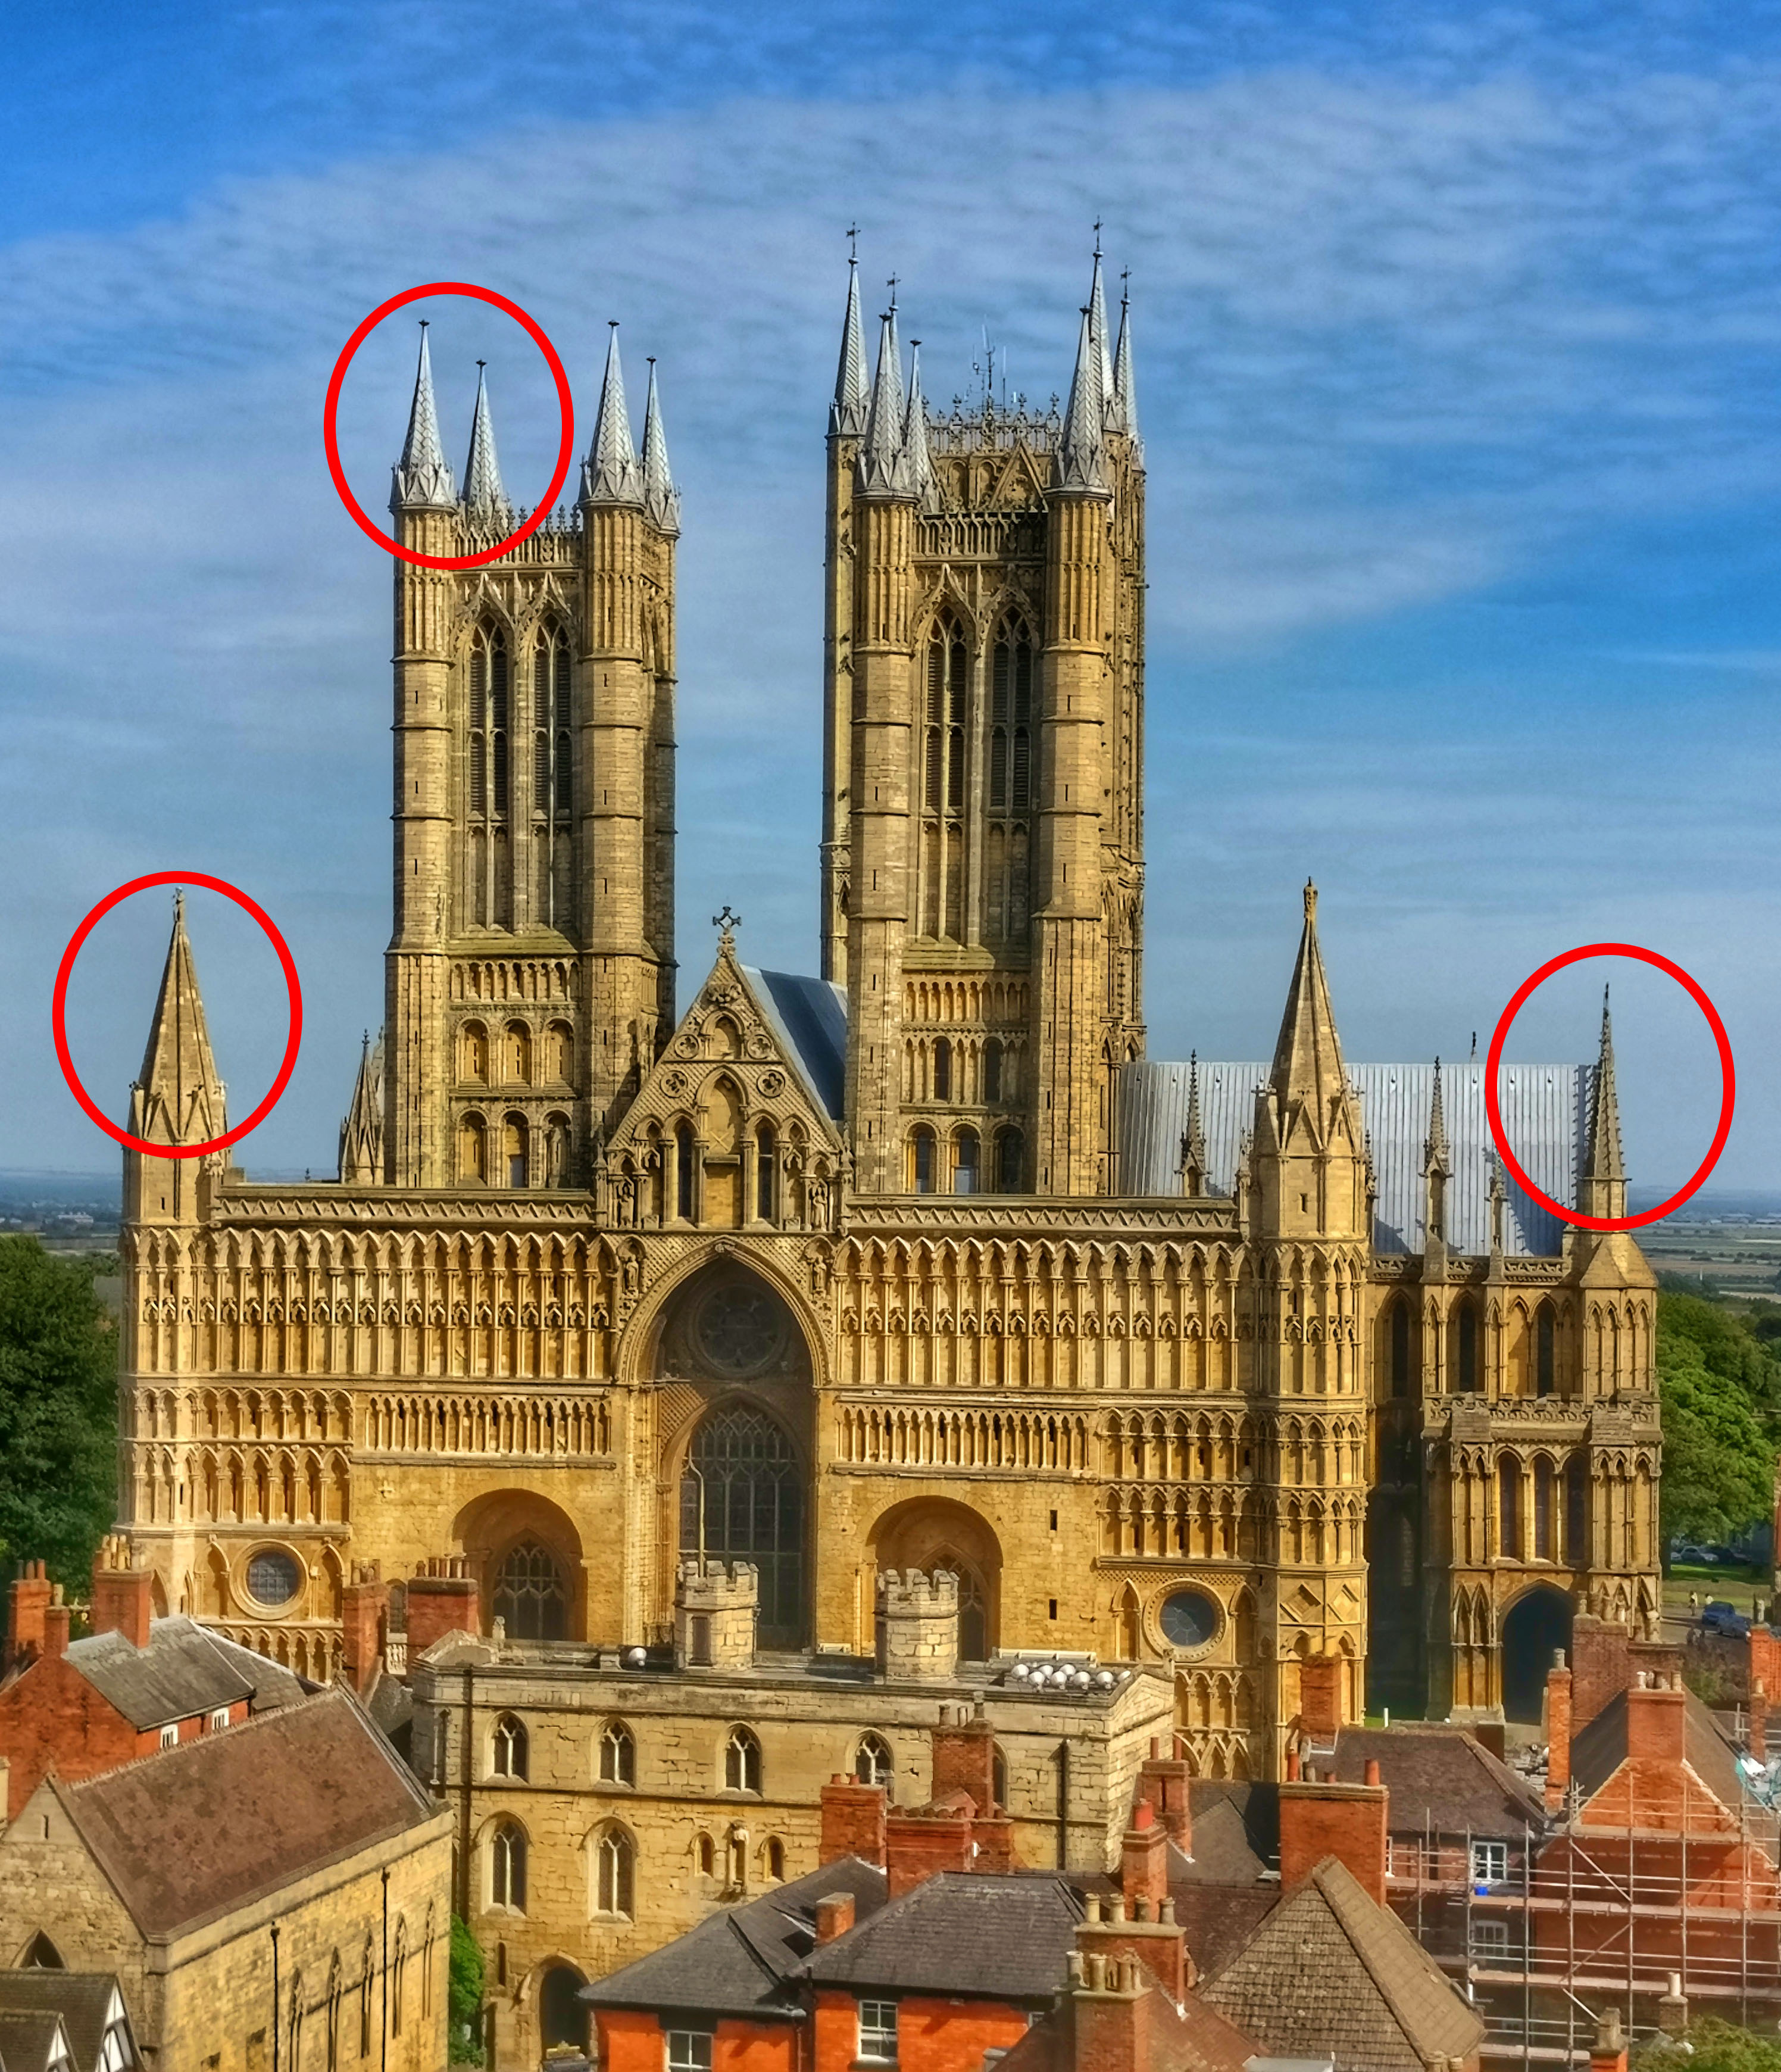
\includegraphics[width=.9\linewidth]{images/LincolnCathedral.jpg}
        \caption{Kathedrale von Lincoln \footnotemark}
    \end{subfigure}
    \caption{Vergleich der verschiedenen architektonischen Einflüsse der Kathedrale von Reims und der Lincoln Kathedrale}
\end{figure}
\footnotetext{Von Johan Bakker, CC BY-SA 3.0,\\\url{https://commons.wikimedia.org/w/index.php?curid=38255047}}
\footnotetext{Von Edbwilco - Eigenes Werk, CC BY-SA 4.0,\\\url{https://commons.wikimedia.org/w/index.php?curid=62286479}}
\subsection{Software-Analogie}
Aber was haben Kathedralen mit der Entwicklung von Softwareprojekten zu tun? Typischerweise bestehen die Teams, die insbesondere große Softwareprojekte umsetzen, aus vielen Entwicklern. Softwareingenieure neigen hierbei auch dazu eine feste Meinung zu haben, wie bestimmte Probleme am besten zu lösen seien. Das ist natürlich menschlich, kann aber dazu führen, dass die Vision des Projektes aus dem Gleichgewicht gerät. Es entsteht eine konzeptionelle Uneinigkeit, welche dazu führen kann, dass es zum Beispiel Probleme bei der Definition von Schnittstellen gibt, was die Entwicklungszeit in die Länge treibt. Es kann aber auch dazu führen, dass der Nutzer bei verschiedenen Komponenten unterschiedlich agieren muss, dadurch verwirrt wird und das Erlernen der Benutzung dieser Software schwerer fällt. Im Vergleich zu Bauprojekten, wie beispielsweise den Kathedralen, liegt die Ursache für diese Uneinigkeit bei Software allerdings nicht bei der Weitergabe des Projekts an nachfolgende Hauptdesigner oder Architekten, sondern an der Einteilung des Designs in viele Aufgaben, die von vielen verschiedenen Menschen bearbeitet werden. \cite{Brooks1975}

\section{Konzeptionelle Integrität}
\subsection{Definition Integrität}
Der Begriff konzeptionelle Integrität ist in keiner Literatur definiert.
Er lässt sich auch in keiner ISO-Norm zur Softwarequalität finden. 
Der Begriff der Integrität lässt sich allerdings definieren.
Seine mehrfach belegte Bedeutung macht ihn zu einem Homonym, da er von Themenfeld zu Themenfeld verschieden ausgelegt werden kann und ist dementsprechend nicht immer auf Anhieb passend zu verstehen. 
Für unsere Begriffe müssen wir ihn aus der lateinischen Sprache übersetzen. Hier bedeutet er \texttt{unversehrt}, \texttt{intakt} oder \texttt{vollständig}. 
Weiter kann man das Wort \texttt{Integrität} mit der Idee des \texttt{Integriert sein} oder \texttt{Eins-sein} in Verbindung bringen.
Die Idee eines Ganzen spiegelt sich in der Art und Weise wieder, wie \texttt{Integrität} verwendet wird, um etwas zu beschreiben, das immer mit den eigenen Erwartungen übereinstimmt.
Wir bezeichnen etwas als begrifflich \texttt{integer}, wenn die aus unserer Erfahrung mit der Sache gebildeten Konzepte die zukünftigen Ereignisse, die mit der Sache verbunden sind, zuverlässig bestimmen können und somit Überraschungen ausgeschlossen werden können.

\subsection{Integer vs. Float}
Wir versuchen anhand dieser beiden Datentypen den Begriff Integrität noch einmal klarer darzustellen. Der Datentyp \texttt{Integer} speichert nur ganze Zahlen, ohne Zwischenwerte. Er bildet also einen bestimmten Zahlenbereich innerhalb der ganzen Zahlen vollständig ab und bietet damit eine gewisse Abgeschlossenheit. Beispielsweise deckt ein \texttt{Integer} mit 32 Bit alle ganze Zahlen zwischen -2.147.483.648 und 2.147.483.647 ab \cite{dewiki:integer}, es ist also vollkommen klar, welche Zahlen von einem 32-Bit \texttt{Integer} dargestellt werden können und welche nicht. Es ist also Integrität gegeben. Das Gegenstück hierzu wäre der Datentyp \texttt{Float}, welcher versucht reelle Zahlen abzubilden. Dieser Datentyp lässt also im Gegensatz zu ganzen Zahlen auch gebrochene Zahlen zu. Dadurch können auch ungenaue Werte entstehen. Eine 32-Bit Fließkommazahl teilt hierfür die Bits in Exponent und Mantisse auf, um dynamisch einen möglichst großen Bereich an Zahlen abzudecken. Dieser Datentyp kann damit auch wesentlich größere Zahlen darstellen, als ein 32-Bit \texttt{Integer}, weist aber genau dann, oder bei Zahlen mit besonders vielen Nachkommastellen, Lücken auf. \cite{dewiki:float} Da reelle Zahlen zu dem \texttt{dicht liegen}, was bedeutet, dass zwischen allen zwei reellen Zahlen immer eine weitere reelle Zahl gefunden werden kann, ist es also auch gar nicht möglich einen Datentyp zu definieren, der einen beliebigen Zahlenbereich in den reellen Zahlen unter Verwendung einer fixen Speichergröße abdeckt. Hier ist also nicht auf Anhieb klar, welche Zahlen nun genau darstellbar sind und welche nicht. Außerdem kann es bei bestimmten Rechnungen zu Rundungsfehlern kommen, weshalb Fließkomma-Datentypen für kritische Daten, wie beispielsweise Kontostände keine Verwendung finden. Bei Fließkommazahlen ist somit nicht automatisch eine Integrität gegeben.

\subsection{Was versteht man unter konzeptioneller Integrität?}
Brooks bringt die \texttt{konzeptionelle Integrität} mit der \texttt{Einheitlichkeit des Designs} in Verbindung, bietet aber leider keine weitere zufriedenstellende Erklärung
dafür, was konzeptionelle Integrität ist. 
Eine naheliegende Definition die wir in unseren deutschen Quellen gefunden haben ist folgende:
Den Grad von Kohäsion und Widerspruchsfreiheit von Anforderungen, die ein System in sich vereinen muss.
Kohäsion ist hierbei ein Maß, das beschreibt, wie eng die Anforderungen der Software zueinander in Beziehung stehen. Ein Programm, dessen Anforderung also möglichst präzise einen gewissen Aufgabenbereich abdecken weist hierbei eine hohe konzeptionelle Integrität auf, während ein Programm, dass möglichst viele Zwecke abdecken soll, die nicht oder kaum miteinander in Verbindung stehen, eine niedrige konzeptionelle Integrität aufweist.

\subsection{Beispiele für konzeptionelle Integrität}
Folgende Beispiele sollen die konzeptionelle Integrität, nach der Definition einer hohen Kohäsion mit Widerspruchsfreiheit, für das Verständnis greifbarer gestalten.

\subsubsection{Kundendaten}
Angenommen, es gibt eine API-Schnittstelle, die das Geburtsdatum eines Kunden in drei Parametern erwartet. Auf dem Kontaktformular der Registrierung gibt es aber nur ein Feld, welches noch dazu kein Format für das Datum an sich vorschreibt. Hier entsteht ein offensichtlicher Widerspruch zwischen den zwei Schnittstellen, welcher für den Entwickler einen erheblichen Aufwand bedeutet, da er entweder das undefinierte Datum in der Eingabemaske in das klar definierte Format der API-Schnittstelle konvertieren, oder die Eingabemaske im Kontaktformular anpassen muss. Hier ist eine konzeptionelle Integrität also nicht gegeben, es entstehen ungeplante Aufgaben und es werden Mehrkosten erzeugt, die man mit einer besseren Planung, beziehungsweise genaueren Anforderungen an das Kontaktformular hätte vermeiden können.

\subsubsection{Bestellsystem}
In einem internationalen Unternehmen, welches sowohl in Deutschland, als auch der Schweiz operiert wird die Anforderung definiert, die Gültigkeit von Postleitzahlen zu prüfen. Hierbei wird ein System von den deutschen Entwicklern umgesetzt und diese implementieren nach bestem Wissen und Gewissen eine Prüfung für eine genau fünfstellige Zahlenkombination. Da das System nun aber auch in der Schweiz funktionieren soll, stößt man bei der Integration dieses Systems auf die Tatsache, dass gültige Postleitzahlen in der Schweiz aus einer vierstelligen Zahlenkombination bestehen. Je nach Umfang des bereits umgesetzten Systems führt dies nun zu tiefgreifenden Änderungen, die durchgeführt werden müssen. Dies hätte beispielsweise mit einer präziseren Definition der Anforderung vermieden werden können.

\subsubsection{Einheitlichkeit}
Bei gängigen Smartphone-Betriebssystemen wie beispielsweise iOS oder Android existieren sogenannte \texttt{Stilvorgaben}. Diese beschreien die Menüführung und das grundsätzliche Layout verschiedener Elemente. Sie werden auch im Betriebssystem durchgehend angewandt. Bestimmte Elemente, wie der Zurück-Knopf, oder ein Burgermenu finden sich immer an derselben Stelle. Richtet sich also ein App-Entwickler nicht an diese \texttt{Stilvorgaben}, treffen die Nutzer nicht an erwarteter Stelle, an diese Elemente und finden diese gegebenenfalls gar nicht. Dies führt zu Verwirrung und damit zu starken Einschränkungen der Benutzbarkeit und Bedienfreude dieser App und sollte natürlich verhindert werden. Hierbei ist auch zu beachten, dass diese \texttt{Stilvorgaben} von Betriebssystem zu Betriebssystem unterschiedlich sind, was insbesondere bei Plattformübergreifenden Apps beachtet werden muss. Auch gilt es zu beachten, dass nicht nur das Layout verschieden sein kann, sondern auch Symbole eine gewisse Bedeutung haben und bei falscher Benutzung falsch oder möglicherweise gar nicht wahrgenommen werden könnten. In modernen Betriebssystemen gibt es auch oft Steuerungsgesten, welche auf Betriebssystemebene funktionieren, um beispielsweise zwischen Apps zu wechseln, diese zu minimieren oder eine Statusleiste einzublenden. Hierbei sollte darauf geachtet werden, dass diese nicht innerhalb der App auch benötigt, oder sogar im Widerspruch zu ihnen stehen, da diese sonst nicht die Erwartung der Nutzer erfüllen, sehr schwer zu entdecken sind oder im Zweifel gar nicht verwendet werden können.  

\subsection{Anwendungs-Suites}
Große Softwareangebote, wie beispielsweise Microsoft Office, oder die Adobe Creative Cloud bieten viele verschiedene Programme, die zueinander in einem gewissen Kontext stehen in einem Gesamtpaket an. Hierbei ist es, im Sinne der konzeptionellen Integrität, dieses Angebot in verschiedene Anwendungen zu unterteilen, statt zu versuchen, eine Art eierlegende Wollmilchsau zu entwickeln. Dies minimiert die Komplexität der Projekte massiv und spart dadurch bei der Konzeption und Implementierung dieser Programme an Zeit. Außerdem ist es dadurch möglich Teams auf die verschiedenen Anwendungen zu verteilen, in denen sich diese dann besser einfinden können. Auch für die Nutzer ist es wesentlich leichter eine dieser Anwendungen zu lernen, beziehungsweise ist die Nutzung wesentlich zweckgebundener, und es muss sich nicht vor dem Start der Arbeit mit diesem Programm durch etliche Menüs geklickt werden, um den gewollten Arbeitsmodus einzustellen. Diese Herangehensweise kann allerdings auch zu Problemen führen, die tatsächlich bei beiden dieser Beispiele gravierend sind. Durch die getrennte Entwicklung dieser Anwendungen kann die Anwendungsübergreifende konzeptionelle Integrität in dem Sinne in Mitleidenschaft gezogen werden, dass beispielsweise verschiedene Menübänder verwendet werden oder identische Funktionen in der einen Software an anderer Stelle gefunden werden, als in der anderen. Bei den meisten Adobe-Creative-Cloud-Anwendungen beispielsweise benötigt man für die Zoom-Funktion die Eingabekombination \texttt{Alt} + \texttt{Mausrad}, während man hierfür bei Adobe-Animate die Kombination \texttt{Strg} + \texttt{Mausrad} verwendet. Dies führt dann natürlich beim Benutzen der einen Software insbesondere dann zu Problemen, wenn man bereits mit der Herangehensweise aus den anderen Anwendungen vertraut ist.

\section{Die Architekten}
Brooks betont in seinem Buch insbesondere, dass die konzeptionelle Integrität diktiert, das Design müsse durch einen einzigen Verstand, oder einer sehr kleinen Zahl sich übereinstimmender Köpfe entstehen. Je mehr Architekten also am Entwurf eines Systems arbeiten, desto eher ist eine konzeptionelle Integrität nicht gegeben.
Selbst 20 Jahren danach, im Jahre 1995, ist Brooks weiterhin von dieser Idee überzeugt: 
\begin{quote}
    Today I am more convinced than ever. Conceptual integrity is central to product quality. Having a system architect is the most important single step toward conceptual integrity. These principles are by no means limited to software systems, but to the design of any complex construct, whether a computer, an airplane, a Strategic Defense Initiative, a Global Positioning System. After teaching a software engineering laboratory more than 20 times, I came to insist that student teams as small as four people choose a manager and a separate architect. Defining distinct roles in such small teams may be a little extreme, but I have observed it to work well and to contribute to design success even for small teams. \cite{wikic2:conceptual_integrity}
\end{quote}
Dies bedeutet also insbesondere, dass man nicht das gesamte Team in den Designprozess einbeziehen sollte. Nur in sehr kleinen Architektenteams kann die Integrität und Qualität des Designs gewährleistet werden.
So ist es unter anderem die Aufgabe der Architekten zu entscheiden:
\begin{itemize}
    \item Welche Features Einzug ins Design finden, welche nachgereicht oder außen vor gelassen werden
    \item Rahmenbedingungen für die Implementierung dieser Features festzulegen
    \item Schnittstellen zwischen den verschiedenen Komponenten zu definieren
    \item Die Komplexität und Kosten gering zu halten
\end{itemize}
Diese Entscheidungen sollte das Architektenteam laut Brooks mit einer gewissen Hoheit treffen und sich eben nicht durch den Einfluss dritter, welche nicht unmittelbar in den Designprozess eingebunden sind von der eigentlichen Vision des Projekts abbringen lassen. 



 \section{Aristocracy and Democracy}
Bei dieser Arbeitsverteilung stellt sich dann schnell die Frage, ob hier eine Zwei-Klassen-Gesellschaft entsteht. Man könnte gar von den \texttt{aristokratischen} Architekten, und den \texttt{pöbelhaften} Programmierern reden. Brooks beleuchtet hierzu insbesondere folgende drei Problemstellungen:
\begin{itemize}
    \item Ist es eine Gefahr, dass die so entstehenden Spezifikationen zu viele Funktionen fordern und damit letztendlich den Preisrahmen sprengen?
    \item Sind die Architekten dann diejenigen, die den ganzen kreativen Spaß haben und somit den Programmierern ihren kreativen Erfindergeist rauben?
    \item Müssen die Programmierer warten, bis das kleine Team von Architekten die Spezifikationen fertiggestellt haben und entsteht hierdurch ein Leerlauf, bei dem diese keine Arbeit haben und dennoch bezahlt werden müssen?
\end{itemize} 
------------------------\\
Der Zeitdruck diktiert jedoch, dass der Systemaufbau viele Hände braucht. Es gibt zwei Möglichkeiten, dieses Dilemma zu lösen. Die erste ist eine sorgfältige Arbeitsteilung zwischen Architektur und Implementierung. Die zweite ist die neue Art der Strukturierung von Programmier-Implementierungsteams, die im vorigen Kapitel besprochen wurde.
Die Trennung von architektonischem Aufwand und Implementierung ist eine sehr wirksame Methode, um konzeptionelle Integrität bei sehr großen Projekten zu erreichen.
Der Architekt eines Systems ist, wie der Architekt eines Gebäudes, der Vertreter des Benutzers. Seine Aufgabe ist es, sein fachliches und technisches Wissen im uneingeschränkten Interesse des Benutzers einzubringen, im Gegensatz zu den Interessen des Verkäufers, des Herstellers usw. Die Architektur muss sorgfältig von der Umsetzung unterschieden werden. Wie Blaauw sagte: "Während die Architektur sagt, was geschieht, sagt die Implementierung, wie es geschieht". Als einfaches Beispiel nennt er eine Uhr, deren Architektur aus dem Zifferblatt, den Zeigern und dem Aufziehknopf besteht. Wenn ein Kind diese Architektur erlernt hat, kann es die Zeit an einer Armbanduhr ebenso leicht ablesen wie an einem Kirchturm. Die Umsetzung und die Verwirklichung beschreiben jedoch, was im Inneren des Gehäuses vor sich geht: die Energieversorgung durch einen von vielen Mechanismen und die Kontrolle der Genauigkeit durch einen von vielen.
------------------------\\

\section{Wischiwaschi}
Die Definition der widerspruchsfreien Anforderungen mit hoher Kohärenz ist schwierig greifbar und macht es problematisch, die Integrität an sich zu messen.
Eine gute Alternative, um die Integrität deutlicher zu machen, wäre die Abwesenheit von dieser festzustellen. Für diese Ausarbeitung haben wir uns für den Begriff 'Wischiwaschi' entschieden, da er auch in unserer Quelle so Verwendung findet und uns auch etwas passend scheint. Indikatoren für Wischiwaschi wären: \\
\begin{itemize}
\item Unklare, widersprüchliche oder mehrdeutige Anforderungen\\
Beispiele für diesen Punkt sind nicht verstandene oder schlecht erklärte User Storys oder Roadmaps.
\item Lange Abstimmungsrunden\\
Gründe wären zu lange Diskussionen, zu viele Verständnisfragen oder Erklärungen zum Projekt
\item Hohe Änderungsraten\\
Wenn sich die Anforderungen in einer hohen Frequenz ändern und der aktuelle Entwicklungsstand dementsprechend aktualisiert werden muss. Beispiele wären von Anfang an unklare Anforderungen, die während der Projektlaufzeit spezifiziert werden.
\item Explodierende Kosten\\
Da die tatsächlichen Kosten die der geplanten Kosten übersteigen ist es möglich, dass die Projektplanung, aufgrund falsch verstandener Anforderungen, schiefgelaufen ist.
\item Projektverzug\\
Gründe können für ein Projektverzug sein, dass die Aufwandsschätzungen, wegen mangel an Verständnis für das Projekt, einfach schlecht waren.
\item Hohe Komplexität\\
Es werden im Team viele Fehler gemacht oder das Verstehen des Projektes scheint schwer zu sein. So steigt die Schieflage immer mehr, je mehr Anforderungen an das Projekt gestellt werden.
\item Schlechte Performance\\
Die Performance ist daher ein Indiz, da das Projekt für die Anwendung ungeeignete oder falsche Werkzeuge nutzt. Mögliche Gründe wären hier zu hohe Änderungsraten, bei denen dann die Werkzeuge nicht optimiert oder ausgetauscht wurden. Auch ein falsches Verständnis vom Projekt könnte eine falsche Annahme der benötigten Mittel herbeiführen.\\
Ein weiterer Grund könnte die unnötige Komplexität des Projektes sein. Funktionen, die einander beeinflussen und somit die Performance reduzieren.
\item Hohe Lernkurve der Anwendung\\
Hohe Lernkurven können passieren aufgrund nicht durchdachtem Design der Anwendung. Ursachen dafür könnten schlecht verstandene Anforderungen, die zu einem schlechten Designkonzept führen.
\end{itemize}
\section{Maßnahmen gegen Wischiwaschi}
Um diese Problematiken zu lösen gibt es mehrere Ansatzpunkte, die wir in Folge erklären.
\subsection{Anforderungsmanagement}
Mit Anforderungsmanagement ist hier die Methode der Aufnahme und Kommunikation der Anforderungen gemeint.
Anforderungen müssen klar, widerspruchsfrei und eindeutig vom Auftraggeber formuliert werden. Sie sind die Grundsteine, damit das Projekt später die konzeptionelle Integrität erfüllt. Um möglichst gute Anforderungen zu erhalten, gibt es Kriterien, die beachtet werden müssen:
\begin{itemize}
\item Abgestimmt:\\
Anforderungen müssen mit allen Stakeholdern abgestimmt werden. Stakeholder müssen die Anforderung als korrekt und notwendig erachten.
\item Eindeutig:\\
Alle Leser müssen beim Studium der Anforderung zum selben Ergebnis kommen. Eine Mehrfachinterpretation sollte nicht möglich sein. Dies ist aufgrund der Mehrdeutigkeit von Sprache sehr schwierig und benötigt viel Erfahrung und Präzision im Schriftlichen. Dies spricht auch für den Bezug auf ein konkretes Lösungsdesign (zum Beispiel in Form eines Prototyps), denn nur dann können die Anforderungen von allen gleich interpretiert werden.
\item Notwendig:\\
Anforderungen müssen den Gegebenheiten im Kontext entsprechen. Eine Gegebenheit kann die Erwartung eines Stakeholders sein oder die API-Spezifikation eines externen Dienstes.
\item Konsistent:\\
Anforderungen müssen sowohl in sich selbst als auch im Vergleich mit anderen Anforderungen konsistent sein. Es darf also keine Widersprüche geben.
\item Prüfbar:\\
Anforderungen müssen überprüfbar sein, damit man später feststellen kann, ob sie umgesetzt wurden. Zur Überprüfung eignen sich Tests oder Messungen.
\item Realisierbar:\\
Nicht jede Anforderung ist im geforderten Budget umsetzbar. Dies ist besonders schwierig, wenn bei den Stakeholdern wenig technisches Verständnis vorhanden ist.
\item Verfolgbar:\\
Der Ursprung der Anforderung muss angegeben werden. Zudem sollte jede Anforderung einen eindeutigen Identifikator haben, damit sie referenziert werden kann.
\item Vollständig:\\
Anforderungen müssen vollständig sein, d. h. die gewünschte Funktionalität in Gänze beschreiben.
\item Verständlich:\\
Die Anforderungen müssen von allen Stakeholdern verstanden werden können. Um dies zu erreichen, sollten sie entweder in der Allgemeinsprache formuliert werden oder es müssen Begriffe in einem Glossar genau erklärt werden.
\end{itemize}
\subsection{Werkzeuge/Tools}
\begin{itemize}
\item Visualisierungen\\
Mithilfe von Grafiken festigt sich das Verständnis für die Anforderungen und klärt somit Widersprüche im Projekt besser auf. Selbst User Storys können helfen, auch wenn sie einem trivial vorkommen kann es jemanden anderem im Team, der nicht auf dem Stand ist, helfen.
\item Application-Lifecycle-Management-Werkzeuge\\
Die Anforderungen müssen möglichst widerspruchsfrei und kohärent bleiben, auch bei Änderungen. Da dies durch viele Informationen und hohe Änderungsfrequenz schwierig ist, können wir uns sogenannte Application-Lifecycle-Management-Werkzeuge (ALM-Werkzeuge) zur Hilfe nehmen. Diese unterstützen die strukturierte Ablage sowie Änderungsprozesse der Informationen gut.\
\item Taxonomie-Software\\
Es hilft eine große Menge von Anforderungen nach zu Strukturen zu definieren. So können über so eine Software diese Anforderungen gruppiert und nach bedarf jederzeit wiedergefunden werden.
\item Wiki-Software\\
So brauchen manche Entwicklungen, vor allem die mittelgroßen bis großen Projekte, mehrere Seiten an Dokumentationen. Teilweise können diese Dokumentationen für die Mitarbeiter unübersichtlich werden und dazu führen, dass die Softwareentwicklung so ins Stocken kommt. Um dies zu verhindern, muss geschaut werden, dass die wichtigen Informationen auf eine zugängliche Art und Weise dokumentiert als auch aktualisiert werden, um Fehlinformationen oder Missinterpretationen zu minimieren.
\end{itemize}
\section{Vorteile hoher konzeptioneller Integrität}
\subsection{Wartbarkeit/Änderbarkeit}
Je konsistenter die Anforderungen und je klarer die Ziele und Epics, desto einfacher ist es, Änderungen an den Anforderungen einzubringen, und die entsprechenden Anpassungen an der Software vorzunehmen. Daraus folgt, dass die Software auch länger in Betrieb gehalten werden kann, da sie sich besser anpassen lässt.
\subsection{Bedienbarkeit/Erlernbarkeit}
Je schlüssiger die Funktionen eines Systems für die Benutzer sind, desto einfacher lassen sie sich auch erlernen.
\subsection{Angepasste Komplexität}
Da Ihr System gut durchdacht ist und eine hohe Kohäsion hat, entsteht keine unnötige Komplexität. Das System kann mit einem optimalen Komplexitätsgrad gebaut werden.
\subsection{Performance}
Unnötige Komplexität in der Source kann Auswirkungen auf die Performance haben. Da keine unnötige Komplexität entstehen muss, ist der Grundstein für eine gute Performance gelegt.
\subsection{Planbarkeit}
Da die Features und ihre Abbildung auf die Software vom Team gut verstanden werden, sind auch die Aufwandschätzungen gut. Die Planbarkeit nimmt zu.
\section{Konzeptionelle Integrität im Scrum-Prozess}
Heutzutage ist Scrum sehr weit verbreitet in der Informatik. Da stellt sich dann natürlich die Frage, auch wenn Brook meinte, dass das Design von einer Gruppe von Architekten designt wird,
ob die konzeptionelle Integrität auch in Scrum erfüllbar wäre? Wir meinen Ja, in einer etwas abgewandelten Form. So gibt es einen Architekten im Team, der meisten spezielle Eigenschaften erfüllt.
\begin{itemize}
    \item Der Architekt hat bezüglich Architektur technische Fragen das letzte Wort im Team \\
    Der Architekt hört sich Vorschläge an, die vom Team kommen und entscheidet ob diese Vorschläge implementiert werden.
    \item Der Architekt gehört zum Projekt und stiftet dem Projekt Nutzen.\\
    Häufig, aber nicht immer, kommt es vor, dass der Architekt im Team selbst ist und sogar auch selbst programmiert.
    In dem Fall ist er auch aktiv an der Entwicklung beteiligt und oft eine Mentorfigur (Senior oder Ausbilder) der mit Tipps und Ratschlägen im Team helfen kann.
    \item Architekt kann auch der Produkt Owner selbst sein
    \item Entscheidungen für das Projekt trifft er selbst unter der Beachtung von Vorgaben.
    Diese Vorgaben können Ressourcen, geplante Termine oder vorhandene Technologien sein.
\end{itemize}
Unabhängig vom Architekt ist Scrum auch ein gutes Konzept, um sowohl im Team als auch außerhalb des Teams transparenz zu schaffen. 
Dies ermöglicht frühzeitig schieflagen im Projekt zu erkennen und zu lösen. Auch erhöht es den Erfolg, durch enge Kommunikation, das Projekt nach einheitlicher zu gestalten.
Folgende Phasen und Hilfsmittel sind dabei wichtig:
\begin{itemize}
    \item Sprint Planning\\
    Am Anfang eines jeden Sprintes wird immer das Warum, Was und Wie geklärt. 
    Es wird jeder früh mit ins Boot geholt und Unklarheiten geklärt.
    Hier können die Teammitglieder sich früh auf gemeinsames nutzen von bestimmten Bibliotheken oder Methoden einigen wie zum Beispiel einheitliche Namenskonventionen.
    \item Daily Scrum\\
    Die täglichen Meetings werden für den Informationsaustausch genutzt. 
    Dadurch ist jeder im Team vom aktuelle Stand im bilde. Probleme können hier frühzeitig kommuniziert und während des Sprintes angepasst werden.
    \item Sprint Review\\
    Am Ende eines Sprintes wird im Review das Ergebniss präsentiert und überprüft, ob erwartete Anforderungen im Sprint Planning erreicht wurden.
     Je nach fortschritt können die Anforderungen, im nächsten Sprint Planning, agil angepasst werden.
    \item Sprint-Retrospektive\\
    Wie in Sprint Review steht auch die Sprint-Retrospektive am Ende eines jeden Sprintes an. Hier wird im Team die vergangene Arbeitweise überdacht und geplant wie diese effektiver wird.
    Dies hat langfristig den Vorteil zwischenmenschliche Probleme im Team als auch Arbeitsweisen für das Projekt zu verbessern und den Erfolg zu steigern.
    \item Produkt Backlog\\
    Im Backlog stehen für jeden die aktuell nötigen Anforderungen transparent für jeden einsehbar. 
    Er wird ständig vom Team aktualisiert und man erkennt daraus den aktuellen Bearbeitungsstatus.
    \item Definition of Done\\
    Um eine Anforderung wirklich als abgeschlossen zu bezeichnen, gibt es Bedingungen die vom Team aufgestellt wurden die vorher erfüllt werden müssen.
    Sie enthalten Qualitätskriterien die vom Team aufgestellt wurden.
     
\end{itemize}
\section{Fazit}

\bibliographystyle{plain}
\bibliography{sources}
\end{document}